\documentclass[11pt]{beamer}
\usepackage[UTF8]{ctex}
\usepackage[utf8]{inputenc}
\usepackage[T1]{fontenc}
\usepackage{lmodern}
\usepackage{amsmath}
\usepackage{amsfonts}
\usepackage{amssymb}
\usepackage{graphicx}
 \usetheme{CambridgeUS}


%%%%%
\usepackage{longtable}
\usepackage{subfigure}
\usepackage{color}
%%%%%
\begin{document}
\author{郭泰彪}
\title{区块链原理及应用}
\subtitle{第0课:课程简介}
\logo{
\includegraphics[scale=0.2]{figures/HNUC.jpeg}}
\institute{湖南工商大学大数据研究院}

%\date{}
%\subject{}
%\setbeamercovered{transparent}
%\setbeamertemplate{navigation symbols}{}
\begin{frame}[plain]
	\maketitle
\end{frame}

\begin{frame}
	\frametitle{目录}
	\tableofcontents[sectionstyle=show,subsectionstyle=show/shaded]
\end{frame}

\section{课程基本信息}
\subsection{课程概述}
\begin{frame}
	\frametitle{课程概述}
	课程设计目标是帮助学生树立分布式整体性世界观,教学大纲将涵盖围绕区块链,通过应用密码学、分布式系统基础、博弈论的基础知识,把区块链作为分布式整体世界观最前沿的创新应用进行系统讲解。课程还将引入区块链智能合约的概念,帮助学生理解区块链编程的理念和应用的方法。特别的,课程还将把区块链隐私保护作为重点进行介绍。

	-

	\footnotesize {
	课程主页(国内):https://taibiaoguo.git{\color{red}ee}.io/blockchain101

	课程主页(国外):https://taibiaoguo.git{\color{red}hub}.io/blockchain101

	代码仓库(国内):https://git{\color{red}ee}.com/taibiaoguo/blockchain101

	代码仓库(国外):https://git{\color{red}hub}.com/taibiaoguo/blockchain101
	}
\end{frame}

\subsection{开课时间和地点}
\begin{frame}
	\frametitle{开课时间和地点}
	\begin{itemize}
		\item 开课时间:2020-2021 第一学期 1-11周 \ \ 周四晚
		\item 上课地点:
		      \begin{enumerate}
			      \item 面授课:E501教室
			      \item 实验课:Exxx机房
		      \end{enumerate}
	\end{itemize}
\end{frame}

\subsection{讲师信息}
\begin{frame}
	\frametitle{讲师信息}
	\begin{figure}
		\centering
		\subfigure{
			\begin{minipage}[ht]{0.65\linewidth}
				\begin{itemize}
					\small{
					\item 姓名:郭泰彪
					\item 办公室:科技楼205
					\item 办公时间:周一至周五 14:00 - 17:00
					\item 邮箱:taibiaoguo@hutb.edu.cn
					\item 工作履历:linkedin.com/in/taibiaoguo
					\item 学术履历:Google Scholar - Taibiao Guo
					\item 开源项目:github.com/TaibiaoGuo
					\item 个人生活:Facebook - 郭泰彪
					      }
				\end{itemize}
				\tiny{Taibiao Guo received the Bachelor degree from China University of Geosciences, Beijing, China, in 2017. He has been involved in the development of blockchain for 3 years in the industry. He is now working in Blockchain Lab, Hunan University of Technology and Business. He is mainly engaged in network attack and defense technology, software and operating system security defect analysis, mobile Internet and Internet of things security technology research. His current research interests include blockchain network architecture and security, secure data storage, secure data computation and user authentication in mobile cloud computing, mobile social network and mobile healthcare with cryptography and machine learning.}
			\end{minipage}
		}%
		\subfigure{
			\begin{minipage}[ht]{0.35\linewidth}
				\centering
				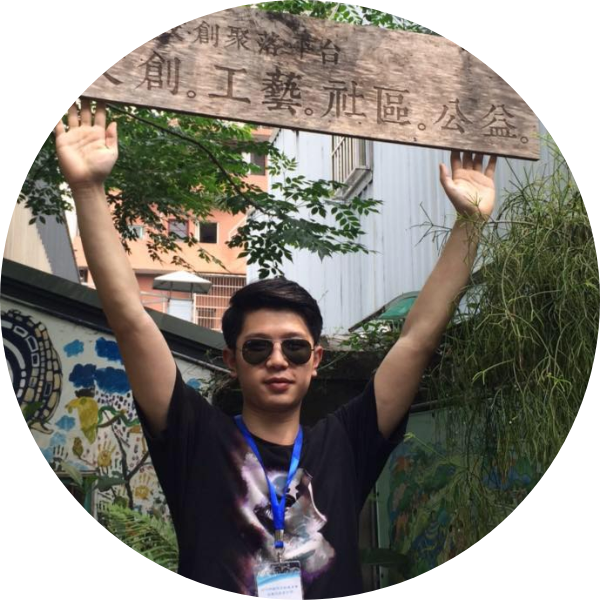
\includegraphics[width=0.9\linewidth]{figures/teacher}
				\label{fig:teacher}
			\end{minipage}%	
		}%
	\end{figure}

\end{frame}


\section{2019-2020疫情期间课程总结}
\subsection{备课总结}
\begin{frame}
	\frametitle{备课总结}
	备课总结:备课不易,费钱、费脑又费事~
	\begin{itemize}
		\item 疫情原因,帮所有学生申请了半年的云服务器,花费10万(阿里巴巴赞助);
		\item 疫情原因,构建了一个课程主页,目前仍在用;
		\item 实验环节,实验工具大概上万行代码;
		\item 查阅了大量文献,掉了点头发(暴风哭泣),消耗了很多咖啡。
	\end{itemize}
\end{frame}
\subsection{学生评价}
\begin{frame}
	\frametitle{学生评价}
	有收获,开眼界,但是课程偏难,命令行是什么鬼!!!

	弹幕节选:
	\begin{itemize}
		\item 好难啊,但是听得很开心!
		\item 原来以为搞区块链的都是金融大佬,非常高大上,非常有钱,em....,上完课,我要把“以为”去掉!
		\item 我一个学设计的,为什么选了这么样一门课?
		\item 所以说,会计要失业了么?律师会失业么?同问,同问!
		\item 就我一个人听不懂么?+1+1+1+1+1+1+1
		\item 老师解释一个名词的过程是引入n个新名词,/(ㄒoㄒ)/~~
		\item 老师什么是命令行,老师命令行怎么删除字符?
		\item 老师妈妈叫我睡觉了,怕我长不高,老师你不困么?
	\end{itemize}
\end{frame}

\subsection{2019-2020疫情期间课程大纲}
\begin{frame}[allowframebreaks]
	\frametitle{2019-2020疫情期间课程大纲}

	\begin{longtable}{llll}
		\hline
		周 & 教学形式 & 授课主题   & 课时标题                                           \\ \hline
		\endfirsthead
		%
		\endhead
		%
		\hline
		\endfoot
		%
		\endlastfoot
		%
		1  & 面授     & 简介       & 《区块链应用场景和前景》                           \\
		1  & 面授     & 简介       & 《区块链发展方向和著名成果简述》                   \\
		2  & 面授     & 博弈论基础 & 《谁在推动区块链系统运行》                         \\
		2  & 面授     & 监管合规   & 《如何"一夜暴富"》                                 \\
		3  & 面授     & 密码学基础 & \small{《非对称加密、Hash、Merkle树和区块的概念》} \\
		3  & 实验     & 密码学基础 & 《实验:openssl、区块生成》                        \\
		4  & 面授     & 分布式基础 & 《P2P网络原理和应用》                              \\
		4  & 实验     & 分布式基础 & 《实验:DHT网络》                                  \\
		5  & 面授     & 分布式基础 & 《分布式共识算法概述》                             \\
		5  & 实验     & 分布式基础 & 《实验:共识算法》                                 \\
		6  & 面授     & 区块链系统 & 《以太坊及其系统架构设计简述》                     \\
		6  & 实验     & 区块链系统 & 《实验:以太坊联盟链部署》                         \\
		7  & 面授     & 智能合约   & 《以太坊智能合约原理及语法1》                      \\
		7  & 面授     & 智能合约   & 《以太坊智能合约语法2》                            \\
		8  & 实验     & 智能合约   & 《实验:以太坊智能合约开发IDE介绍》                \\
		8  & 实验     & 智能合约   & 《实验:以太坊智能合约部署和调用》                 \\
		9  & 实验     & 应用开发   & 《实验:博客框架部署及使用》                       \\
		9  & 实验     & 应用开发   & 《实验:部署自己的博客系统》                       \\
		10 & 实验     & 应用开发   & 《实验:编写数字积分打赏合约》                     \\
		10 & 实验     & 应用开发   & 《实验:区块链浏览器使用介绍》                     \\
		11 & 实验     & 应用开发   & 《实验:制作一个数字积分打赏插件》                 \\
		11 & 实验     & 应用开发   & \small{《实验:将付费阅读博客部署到公有云平台》}   \\
		12 & 其他     & 结课答疑   & 结课答疑                                           \\ \hline
	\end{longtable}
\end{frame}

\subsection{学生学习情况总结}
\begin{frame}
	\frametitle{学生学习情况总结}
	学生学习情况总结:

	通过结课报告,可以分析出大部分的学生能掌握区块链的性质和应用场景,

	小部分学生能理解区块链的密码学、分布式系统、博弈论原理。
\end{frame}

\section{2020-2021学期课程安排}
\subsection{本学期课程的变化}
\begin{frame}
	\frametitle{本学期课程的变化}
	\begin{itemize}
		\item 弱化编程课程的时长;
		\item 简化区块链原理的难度;
		\item 强化区块链应用和趋势的介绍;
	\end{itemize}
\end{frame}

\subsection{成绩计算方法}
\begin{frame}
	\frametitle{成绩计算方法}
	本课程学分2分,采用100分制计分,分数计算标准如下:
	\begin{itemize}
		\item 平时成绩44分:
		      \begin{itemize}
			      \item 课堂考勤20分。考勤抽查,一次未到扣5分,最多扣20分;
			      \item 课后作业24分。按作业要求,在每次作业截止时间前提交有效,共4次,一次作业6分;
		      \end{itemize}
		\item 课堂讨论26分。在12周课程结束前,通过课堂讨论区\footnote{github.com/taibiaoguo/blockchain101}的Issues面板提出或回复问题得分,禁止灌水;

		      其中,提出一个有效问题3分,最多9分;产生一个有效回复3分,最多15分;关注(Star)本课程对应Github项目blockchain101得2分;
		\item 结课成果30分。可自由通过成果展示、结课论文、PPT展示、专利申请书等多种方式完成结课成果,老师将根据成果水平进行评分。
	\end{itemize}
	\footnote{为方便统计,提问和回答必须在正文末尾新起一行附上名字最后一位和学号后三位,如:婷019才算有效。课堂讨论溢出得分最多可抵扣5分课堂考勤扣分}
\end{frame}

\subsection{得分点清单}
\begin{frame}
	\frametitle{得分点清单}
	\begin{itemize}
		\item 平时上课签到20分;
		\item 课后作业24分;
		\item 课堂讨论区提问9分;
		\item 课堂讨论区回复15分;
		\item 关注本课程Github上的项目blockchain101 \ 2分;
		\item 结课成果30分;
	\end{itemize}
	此外,课堂讨论区溢出得分可抵扣5分上课签到扣分。
\end{frame}

\subsection{课程形式}
\begin{frame}
	\frametitle{课程形式}
	该课程的学习形式包括:
	\begin{itemize}
		\item 阅读和评论:课程会有阅读任务。您应该在上课前一天完成阅读并评论材料;
		\item 小组讨论:本课程老师与学生在课堂会积极互动,各位可以在课堂上积极提出关键的概念,想法和直觉,并共同处理困难的资料;
		\item 上机实践:本课程会包含上机实践内容,不需要计算机基础;
		\item 课后作业:习题会在附在课程资料中,习题需要在每周日12:00前通过邮件发送给老师。
	\end{itemize}
\end{frame}

\subsection{课程目标}
\begin{frame}
	\frametitle{课程目标}
	在课程结束时,希望大家都能:
	\begin{itemize}
		\item 可以向其他人解释区块链的概念和应用场景;
		\item 熟悉区块链的现状和未来发展方向;
		\item 了解区块链的原理;
		\item 能够利用搜索引擎、学术论文、博客、论坛等途径对区块链进行深入学习。
	\end{itemize}
\end{frame}

\subsection{提问方式}
\begin{frame}
	\frametitle{提问方式}
	如果您在本课程学习过程中有任何不明白的地方,可以通过Github Issue的方式进行提问,鼓励使用Github Issue的方式进行提问,也可以在课上或课后与老师进行讨论。
\end{frame}

\subsection{专利奖励}
\begin{frame}
	\frametitle{专利奖励}
	为了鼓励创新,本课程结课报告若具有创新性并在申报后获得发明专利授权,结课报告递交者可获得区块链课程的科研奖励:1万元人民币整。细则如下(试行):
	\begin{enumerate}
		\item 学生结课时以发明专利申请书的形式撰写结课报告;
		\item 授课老师进行初审,对潜在发明给予修改意见,并指导学生申请发明专利,支付发明专利代理费用;
		\item 专利在下学期开始前拿到发明专利申请号,并在成功获得专利授权后,学生可一次性获得本课程的科研奖励1万元人民币整。
	\end{enumerate}
\end{frame}
\end{document}